\documentclass[nooutcomes]{ximera}
%\documentclass[space,handout,nooutcomes]{ximera}

\usepackage{epsfig}

\graphicspath{
  {./}
  {figures/}
  {../laode}
  {../laode/figures}
}

\usepackage{epstopdf}
\epstopdfsetup{outdir=./}

\usepackage{morewrites}
\makeatletter
\newcommand\subfile[1]{%
\renewcommand{\input}[1]{}%
\begingroup\skip@preamble\otherinput{#1}\endgroup\par\vspace{\topsep}
\let\input\otherinput}
\makeatother

\newcommand{\EXER}{}
\newcommand{\includeexercises}{\EXER\directlua{dofile(kpse.find_file("exercises","lua"))}}

\newenvironment{computerExercise}{\begin{exercise}}{\end{exercise}}

%\newcounter{ccounter}
%\setcounter{ccounter}{1}
%\newcommand{\Chapter}[1]{\setcounter{chapter}{\arabic{ccounter}}\chapter{#1}\addtocounter{ccounter}{1}}

%\newcommand{\section}[1]{\section{#1}\setcounter{thm}{0}\setcounter{equation}{0}}

%\renewcommand{\theequation}{\arabic{chapter}.\arabic{section}.\arabic{equation}}
%\renewcommand{\thefigure}{\arabic{chapter}.\arabic{figure}}
%\renewcommand{\thetable}{\arabic{chapter}.\arabic{table}}

%\newcommand{\Sec}[2]{\section{#1}\markright{\arabic{ccounter}.\arabic{section}.#2}\setcounter{equation}{0}\setcounter{thm}{0}\setcounter{figure}{0}}
  
\newcommand{\Sec}[2]{\section{#1}}

\setcounter{secnumdepth}{2}
%\setcounter{secnumdepth}{1} 

%\newcounter{THM}
%\renewcommand{\theTHM}{\arabic{chapter}.\arabic{section}}

\newcommand{\trademark}{{R\!\!\!\!\!\bigcirc}}
%\newtheorem{exercise}{}

\newcommand{\dfield}{{\sf dfield9}}
\newcommand{\pplane}{{\sf pplane9}}
\newcommand{\PPLANE}{{\sf PPLANE9}}

% BADBAD: \newcommand{\Bbb}{\bf}

\newcommand{\R}{\mbox{$\Bbb{R}$}}
\newcommand{\C}{\mbox{$\Bbb{C}$}}
\newcommand{\Z}{\mbox{$\Bbb{Z}$}}
\newcommand{\N}{\mbox{$\Bbb{N}$}}
\newcommand{\D}{\mbox{{\bf D}}}
\usepackage{amssymb}
%\newcommand{\qed}{\hfill\mbox{\raggedright$\square$} \vspace{1ex}}
%\newcommand{\proof}{\noindent {\bf Proof:} \hspace{0.1in}}

\newcommand{\setmin}{\;\mbox{--}\;}
\newcommand{\Matlab}{{M\small{AT\-LAB}} }
\newcommand{\Matlabp}{{M\small{AT\-LAB}}}
\newcommand{\computer}{\Matlab Instructions}
\newcommand{\half}{\mbox{$\frac{1}{2}$}}
\newcommand{\compose}{\raisebox{.15ex}{\mbox{{\scriptsize$\circ$}}}}
\newcommand{\AND}{\quad\mbox{and}\quad}
\newcommand{\vect}[2]{\left(\begin{array}{c} #1_1 \\ \vdots \\
 #1_{#2}\end{array}\right)}
\newcommand{\mattwo}[4]{\left(\begin{array}{rr} #1 & #2\\ #3
&#4\end{array}\right)}
\newcommand{\mattwoc}[4]{\left(\begin{array}{cc} #1 & #2\\ #3
&#4\end{array}\right)}
\newcommand{\vectwo}[2]{\left(\begin{array}{r} #1 \\ #2\end{array}\right)}
\newcommand{\vectwoc}[2]{\left(\begin{array}{c} #1 \\ #2\end{array}\right)}

\newcommand{\ignore}[1]{}


\newcommand{\inv}{^{-1}}
\newcommand{\CC}{{\cal C}}
\newcommand{\CCone}{\CC^1}
\newcommand{\Span}{{\rm span}}
\newcommand{\rank}{{\rm rank}}
\newcommand{\trace}{{\rm tr}}
\newcommand{\RE}{{\rm Re}}
\newcommand{\IM}{{\rm Im}}
\newcommand{\nulls}{{\rm null\;space}}

\newcommand{\dps}{\displaystyle}
\newcommand{\arraystart}{\renewcommand{\arraystretch}{1.8}}
\newcommand{\arrayfinish}{\renewcommand{\arraystretch}{1.2}}
\newcommand{\Start}[1]{\vspace{0.08in}\noindent {\bf Section~\ref{#1}}}
\newcommand{\exer}[1]{\noindent {\bf \ref{#1}}}
\newcommand{\ans}{\textbf{Answer:} }
\newcommand{\matthree}[9]{\left(\begin{array}{rrr} #1 & #2 & #3 \\ #4 & #5 & #6
\\ #7 & #8 & #9\end{array}\right)}
\newcommand{\cvectwo}[2]{\left(\begin{array}{c} #1 \\ #2\end{array}\right)}
\newcommand{\cmatthree}[9]{\left(\begin{array}{ccc} #1 & #2 & #3 \\ #4 & #5 &
#6 \\ #7 & #8 & #9\end{array}\right)}
\newcommand{\vecthree}[3]{\left(\begin{array}{r} #1 \\ #2 \\
#3\end{array}\right)}
\newcommand{\cvecthree}[3]{\left(\begin{array}{c} #1 \\ #2 \\
#3\end{array}\right)}
\newcommand{\cmattwo}[4]{\left(\begin{array}{cc} #1 & #2\\ #3
&#4\end{array}\right)}

\newcommand{\Matrix}[1]{\ensuremath{\left(\begin{array}{rrrrrrrrrrrrrrrrrr} #1 \end{array}\right)}}

\newcommand{\Matrixc}[1]{\ensuremath{\left(\begin{array}{cccccccccccc} #1 \end{array}\right)}}



\renewcommand{\labelenumi}{\theenumi}
\newenvironment{enumeratea}%
{\begingroup
 \renewcommand{\theenumi}{\alph{enumi}}
 \renewcommand{\labelenumi}{(\theenumi)}
 \begin{enumerate}}
 {\end{enumerate}\endgroup}

\newcounter{help}
\renewcommand{\thehelp}{\thesection.\arabic{equation}}

%\newenvironment{equation*}%
%{\renewcommand\endequation{\eqno (\theequation)* $$}%
%   \begin{equation}}%
%   {\end{equation}\renewcommand\endequation{\eqno \@eqnnum
%$$\global\@ignoretrue}}

%\input{psfig.tex}

\author{Martin Golubitsky and Michael Dellnitz}

%\newenvironment{matlabEquation}%
%{\renewcommand\endequation{\eqno (\theequation*) $$}%
%   \begin{equation}}%
%   {\end{equation}\renewcommand\endequation{\eqno \@eqnnum
% $$\global\@ignoretrue}}

\newcommand{\soln}{\textbf{Solution:} }
\newcommand{\exercap}[1]{\centerline{Figure~\ref{#1}}}
\newcommand{\exercaptwo}[1]{\centerline{Figure~\ref{#1}a\hspace{2.1in}
Figure~\ref{#1}b}}
\newcommand{\exercapthree}[1]{\centerline{Figure~\ref{#1}a\hspace{1.2in}
Figure~\ref{#1}b\hspace{1.2in}Figure~\ref{#1}c}}
\newcommand{\para}{\hspace{0.4in}}

\usepackage{ifluatex}
\ifluatex
\ifcsname displaysolutions\endcsname%
\else
\renewenvironment{solution}{\suppress}{\endsuppress}
\fi
\else
\renewenvironment{solution}{}{}
\fi

%\ifxake
%\newenvironment{matlabEquation}{\begin{equation}}{\end{equation}}
%\else
\newenvironment{matlabEquation}%
{\let\oldtheequation\theequation\renewcommand{\theequation}{\oldtheequation*}\begin{equation}}%
  {\end{equation}\let\theequation\oldtheequation}
%\fi

\makeatother



\title{Similar Right Triangles}
\author{Brad Findell}
\begin{document}
\begin{abstract}
Proofs. 
\end{abstract}
\maketitle

\begin{problem}
Adapted from Ohio's 2017 Geometry released item 17.

\begin{image}
\definecolor{qqwuqq}{rgb}{0.,0.39215,0.}
\definecolor{uuuuuu}{rgb}{0.2667,0.2667,0.2667}
\definecolor{qqqqff}{rgb}{0.,0.,1.}
\begin{tikzpicture}[line cap=round,line join=round,>=triangle 45,x=1.0cm,y=1.0cm]
%\clip(-0.75,-1) rectangle (2.9,3.5);
\clip(-3,-.1) rectangle (5,3.3);
\draw[line width=0.8pt,color=qqwuqq,fill=qqwuqq,fill opacity=0.1] (0.,0.) -- (0.,0.25) -- (0.25,0.25) -- (0.25,0.) -- cycle;
\draw[line width=0.8pt,color=qqwuqq,fill=qqwuqq,fill opacity=0.1] (1.2457,1.1314) -- (1.0373,0.9925) -- (1.1762,0.7842) -- (1.3846,0.9231) -- cycle;
\draw[line width=0.8pt,color=qqwuqq,fill=qqwuqq,fill opacity=0.1] (1.1762,0.7842) -- (1.3152,0.5758) -- (1.5235,0.7147) -- (1.3846,0.9231) -- cycle;
\draw [line width=0.8pt] (0.,0.)-- (2.,0.);
\draw [line width=0.8pt] (0.,3.)-- (0.,0.);
\draw [line width=0.8pt] (0.,3.)-- (2.,0.);
\draw [line width=0.8pt,dash pattern=on 3pt off 3pt] (0.,0.)-- (1.3846,0.9231);
\begin{scriptsize}
\draw [fill=qqqqff] (0.,0.) circle (1.2pt);
\draw[color=qqqqff] (-0.25,0.15) node {$A$};
\draw [fill=qqqqff] (2.,0.) circle (1.2pt);
\draw[color=qqqqff] (2.20,0.15) node {$B$};
\draw [fill=qqqqff] (0.,3.) circle (1.2pt);
\draw[color=qqqqff] (0.22,3.20) node {$C$};
\draw [fill=uuuuuu] (1.3846,0.9231) circle (1.2pt);
\draw[color=uuuuuu] (1.58,1.10) node {$D$};
\end{scriptsize}
\end{tikzpicture}
\end{image}
 
%\begin{image}
%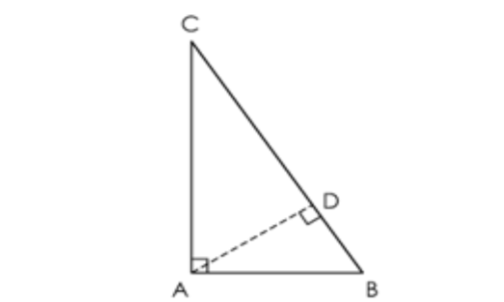
\includegraphics{Q17.png}
%\end{image}
Complete the following proof that $\triangle DAC$ is similar to $\triangle DBA$:
% The 2017 EOC item prompts for ``AA postulate,'' but AA is not a postulate.
 
\begin{enumerate}
\item $\triangle DBA\sim \triangle \answer[format=string]{ABC}$ by \wordChoice{\choice[correct]{AA similarity}\choice{CPCTC}\choice{right triangle similarity}} because they share $\angle B$ and they each have a right angle.
 
\item $\triangle DAC\sim \triangle \answer[format=string]{ABC}$ for the same reason because they share \wordChoice{\choice{$\angle A$}\choice{$\angle B$}\choice[correct]{$\angle C$}} and they each have a right angle.
 
\item $\triangle DAC\sim \triangle DBA$ because 
\wordChoice{\choice{CPCTC}\choice{right triangle similarity}\choice[correct]{they are both similar to$\triangle ABC$}}.
\end{enumerate}
 
\end{problem}


\begin{problem}
A different proof, also adapted from Ohio's 2017 Geometry released item 17. 

\begin{image}
\definecolor{qqwuqq}{rgb}{0.,0.39215,0.}
\definecolor{uuuuuu}{rgb}{0.2667,0.2667,0.2667}
\definecolor{qqqqff}{rgb}{0.,0.,1.}
\begin{tikzpicture}[line cap=round,line join=round,>=triangle 45,x=1.0cm,y=1.0cm,scale=0.8]
%\clip(-0.75,-1) rectangle (2.9,3.5);
%\clip(-2,-1) rectangle (4,3.5);
\draw[line width=0.8pt,color=qqwuqq,fill=qqwuqq,fill opacity=0.1] (0.,0.) -- (0.,0.25) -- (0.25,0.25) -- (0.25,0.) -- cycle; 
\draw[line width=0.8pt,color=qqwuqq,fill=qqwuqq,fill opacity=0.1] (1.2457,1.1314) -- (1.0373,0.9925) -- (1.1762,0.7842) -- (1.3846,0.9231) -- cycle; 
\draw[line width=0.8pt,color=qqwuqq,fill=qqwuqq,fill opacity=0.1] (1.1762,0.7842) -- (1.3152,0.5758) -- (1.5235,0.7147) -- (1.3846,0.9231) -- cycle; 
\draw [line width=0.8pt] (0.,0.)-- (2.,0.);
\draw [line width=0.8pt] (0.,3.)-- (0.,0.);
\draw [line width=0.8pt] (0.,3.)-- (2.,0.);
\draw [line width=0.8pt,dash pattern=on 3pt off 3pt] (0.,0.)-- (1.3846,0.9231);
\begin{scriptsize}
\draw [fill=qqqqff] (0.,0.) circle (1.2pt);
\draw[color=qqqqff] (-0.25,0.15) node {$A$};
\draw [fill=qqqqff] (2.,0.) circle (1.2pt);
\draw[color=qqqqff] (2.20,0.15) node {$B$};
\draw [fill=qqqqff] (0.,3.) circle (1.2pt);
\draw[color=qqqqff] (0.22,3.20) node {$C$};
\draw [fill=uuuuuu] (1.3846,0.9231) circle (1.2pt);
\draw[color=uuuuuu] (1.58,1.10) node {$D$};
\end{scriptsize}
\end{tikzpicture}
\end{image}

%\begin{image}
%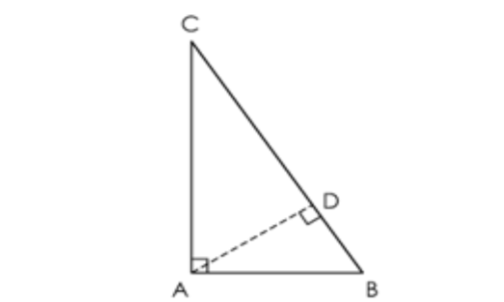
\includegraphics{Q17.png}
%\end{image}
Complete the following proof that $\triangle DAC$ is similar to $\triangle DBA$: 
% The 2017 EOC item prompts for ``AA postulate,'' but AA is not a postulate.

\begin{enumerate}
\item $\angle B$ and $\angle BAD$ are $\answer[format=string]{complementary}$ because they are acute angles in a right triangle. 

\item $\angle DAC$ and $\angle BAD$ are complementary because they are adjacent angles that form $\angle BAC$, which is \wordChoice{\choice[correct]{right}\choice{acute}\choice{obtuse}}.  

\item $\angle B \cong \angle DAC$ because they are both complementary to $\angle BAD$.  

\item $\triangle DAC\sim \triangle DBA$ by \wordChoice{\choice[correct]{AA similarity}\choice{CPCTC}\choice{right triangle similarity}} because $\angle B \cong \angle DAC$ and they each have a right angle.
\end{enumerate}

\end{problem}


\end{document}
